\documentclass[
  aps,
  reprint,
  superscriptaddress,
  floatfix,
  nofootinbib,
  longbibliography
]{revtex4-2}

\usepackage{amsmath,amssymb}
\usepackage{graphicx}
\usepackage{bm}
\usepackage{xcolor}
\usepackage{tikz}
\usetikzlibrary{calc,positioning,arrows.meta}
\usepackage{hyperref}

\hypersetup{
  colorlinks=true,
  linkcolor=blue,
  citecolor=blue,
  urlcolor=blue
}

% --- convenience macros -------------------------------------------------
\newcommand{\R}{\mathbb{R}}
\newcommand{\E}{\mathbb{E}}
\newcommand{\Prob}{\mathbb{P}}
\newcommand{\Sph}[1]{S^{#1}}
\newcommand{\deff}{d_{\mathrm{eff}}}
\newcommand{\meff}{m_{\mathrm{eff}}}
\newcommand{\sint}{\sigma_{\mathrm{int}}}
\newcommand{\Eint}{E_{\mathrm{int}}}
\newcommand{\T}{^{\mathsf{T}}}
\newcommand{\opnorm}[1]{\lVert #1 \rVert_{\mathrm{op}}}
\newcommand{\norm}[1]{\lVert #1 \rVert}
\newcommand{\ReLU}{\mathrm{ReLU}}
\newcommand{\hpar}{h_{\parallel}}
\newcommand{\hperp}{h_{\perp}}

\DeclareMathOperator*{\argmax}{arg\,max}
\DeclareMathOperator{\spanop}{span}
\DeclareMathOperator{\Var}{Var}

\begin{document}

\title{Semantic Concurrency Limits in Large Language Models}

\author{Karl Svozil}
\email{karl.svozil@tuwien.ac.at}
\affiliation{Institute for Theoretical Physics, TU Wien,
Wiedner Hauptstra\ss{}e 8--10/136, 1040 Vienna, Austria}

\date{\today}

\begin{abstract}
High-dimensional embedding spaces can host many semantic directions
with small mutual overlap. But small overlaps are not zero: when many
directions are jointly active, their residual interference accumulates
and limits what a finite readout channel can recover. We formulate this
as a distinction between \emph{kinetic capacity}---what the geometry
can host---and \emph{epistemic accessibility}---what readout can
recover. The two sides are summarized by
$N\lesssim\exp(c\,\deff\,\varepsilon^{2})$ for coexistence and
$\sint\sim\sqrt{k/\deff}$ for simultaneous readout. Thus dimension acts
not merely as storage capacity but as semantic concurrency bandwidth.
On this geometric foundation we propose a separate hypothesis: some
polysemous tokens may be organized around stable token-associated
hinge directions, with sense information carried by low-dimensional
subspaces in the hinge-perpendicular carrier. The capacity/accessibility
distinction is the main claim; the hinge hypothesis is a stronger,
separately falsifiable empirical proposal.
\end{abstract}

\maketitle

% ======================================================================
\section{Introduction}
\label{sec:intro}
% ======================================================================

A finite-dimensional activation space faces a simple tension. High
dimension lets many semantic features coexist as nearly orthogonal
directions. Finite readout prevents too many of them from being
simultaneously recovered from one channel. This paper makes that
tension quantitative.

The two sides obey different scalings. On the capacity side,
concentration of measure permits exponentially many candidate semantic
directions with pairwise overlap at most $\varepsilon$,
%
\begin{equation}
\label{eq:intro-capacity}
N\lesssim \exp(c\,\deff\,\varepsilon^{2}).
\end{equation}
%
On the readout side, the same small residual overlaps add in quadrature
over an active set of size $k$, giving an interference scale
%
\begin{equation}
\label{eq:intro-readout}
\sint\sim\sqrt{k/\deff}.
\end{equation}
%
The first relation is an existential packing estimate. The second is a
typical-case readout-noise estimate. Together they say that dimension
is a \emph{semantic concurrency bandwidth}: it does not mainly limit how
many meanings can be geometrically stored, but how many independently
recoverable semantic components can be jointly active.

Polysemy is the cleanest example. A single lexical item, such as
``bank'', can access several mutually exclusive meanings, only one of
which is selected in a given context. The same tension appears more
generally in feature superposition, role binding, and compositional
semantics~\cite{mikolov2013}: many latent semantic degrees of freedom
must coexist, while only a context-selected subset is read out. We use
polysemy as a controlled entry point because it makes contextual
selection explicit. In lexical semantics, polysemy is distinguished
from homonymy by the relatedness of senses~\cite{pustejovsky1995}.
Modern Transformer-based LLMs implement contextual selection through
dynamic contextual embeddings: a token representation is repeatedly
transformed by self-attention and MLP layers as it absorbs information
from its sentential environment~\cite{Vaswani-2017-Attention}.

The paper makes two claims. The first is the geometric capacity claim:
concentration permits large semantic capacity, while accumulated
interference limits simultaneous accessibility. This claim is
architecture-independent. The second is a stronger organizational
hypothesis: for some canonically polysemous tokens, readout may be
structured around a stable token-associated \emph{hinge} direction,
with sense information carried by low-dimensional subspaces in its
orthogonal complement. The hinge hypothesis is not implied by
concentration geometry. It is an empirical proposal, and
Sec.~\ref{sec:predictions} states how it can fail.

A serious caveat is effective dimension. Trained representations are
often anisotropic: they occupy a narrow cone rather than the full
ambient space. The dimension controlling concentration is therefore
not necessarily the raw embedding dimension $d$, but an effective
dimension $\deff$. If $\deff$ is small, the capacity claim weakens
accordingly. For example, at $\deff\sim 50$ and $\varepsilon=0.1$, the
exponent $c\deff\varepsilon^{2}$ is only a small constant. The framework
therefore applies to the approximately isotropic geometry actually used
by the representation, possibly after whitening or restriction to a
participation subspace. Determining which layers, models, and
preprocessing regimes admit a meaningful $\deff$ is an empirical
priority.

The hinge hypothesis has a narrower domain. It is meant for
canonically polysemous tokens with established sense inventories, such
as WordNet-, OntoNotes-, SemCor-, or WiC-style sense
distinctions~\cite{pilehvar2019wic} with enough contextual instances
for testing. Failure on a representative sample, against the controls
in Sec.~\ref{sec:predictions}, would count against hinge anchoring even
if the broader capacity/accessibility picture survives.

The proposal is adjacent to the superposition hypothesis in mechanistic
interpretability~\cite{elhage2022superposition}, according to which neural networks
represent more features than they have neurons by packing features into
nearly orthogonal directions. The present paper separates the
geometric background from a possible semantic organization within it.
The general superposition picture concerns an overcomplete dictionary
of feature directions and sparse active sets. The hinge picture adds
the more specific possibility that some contextual readout is organized
around stable token-associated directions.

Section~\ref{sec:concentration} develops the capacity framework:
quasi-orthogonality, L\'evy's lemma, exponential packing, and the
kinetic/epistemic distinction. Section~\ref{sec:hinge} introduces the
hinge-and-frame hypothesis and its relation to dynamic contextual
embeddings. Section~\ref{sec:attention} connects the picture to
attention as soft routing rather than literal frame reconstruction.
Section~\ref{sec:discussion} discusses superposition, sparse
autoencoders, limitations, empirical tests, and the limited quantum
analogy.

{Notation.}
Throughout, $\R^{d}$ is Euclidean $d$-space with inner product $u\T v$
and norm $\norm{v}=\sqrt{v\T v}$; $\Sph{d-1}=\{v\in\R^{d}:\norm{v}=1\}$
is the unit sphere; $I$ is the identity matrix; $\opnorm{\cdot}$ is the
operator norm; $A\succeq0$ means positive semidefinite; and $\Prob$ and
$\E$ denote probability and expectation under the uniform measure on
the relevant sphere unless stated otherwise. Universal positive
constants are denoted $c,c'$, possibly changing from line to line.
The symbol $\deff$ denotes the effective dimension controlling
concentration in the representation being probed.

% ======================================================================
\section{Concentration geometry and capacity}
\label{sec:concentration}
% ======================================================================

This section is architecture-independent. It gives the geometric
capacity constraint on which the later hinge hypothesis builds.

\subsection{Quasi-orthogonality}
\label{sec:quasiortho}

Let $v_{1},\dots,v_{N}\in\R^{d}$ be unit vectors. Strict orthogonality,
$v_i\T v_j=0$ for $i\neq j$, allows at most $N=d$ such vectors. Semantic
encoding does not require exact orthogonality. It requires approximate
distinguishability. We therefore call a family
$\varepsilon$-quasi-orthogonal if
%
\begin{equation}
\label{eq:quasiortho}
|v_i\T v_j|\le \varepsilon,\qquad i\neq j .
\end{equation}
%
This is the relevant notion for high-dimensional feature storage:
small overlap is tolerable, provided readout can absorb the resulting
interference.

\subsection{L\'evy's lemma and linear overlaps}
\label{sec:levy}

High-dimensional spheres make quasi-orthogonality generic.

%\paragraph*{Heuristic concentration argument.}
The mechanism is already visible before invoking the formal lemma.  Let
\[
        x=(x_1,\ldots,x_d)\in\R^d
\]
be a unit vector chosen without a preferred direction.  Then
\[
        x_1^2+\cdots+x_d^2=1 .
\]
Rotational invariance suggests that the norm is spread over the available
coordinates, so a typical coordinate weight is of order $1/d$.  Now fix a
unit direction $u$.  By rotational invariance one may choose coordinates so
that $u=e_1$.  The squared overlap with the random direction is then
\[
        |u\T x|^2=x_1^2 .
\]
Thus the overlap with any fixed direction is typically of order $d^{-1/2}$
in amplitude, or $1/d$ in squared amplitude.  A macroscopic overlap
$|u\T x|>\varepsilon$ therefore requires one coordinate to carry an
anomalously large fraction of the total norm.  In high dimension such an
event is exponentially unlikely.

The same intuition appears particularly transparently in the complex
Hilbert-space analogue.  If $\psi\in\mathbb{C}^D$ is Haar-random and
$\phi$ is fixed, unitary invariance permits the choice $\phi=e_1$, so
\[
        |\langle\phi,\psi\rangle|^2=|\psi_1|^2 .
\]
For a Haar-random complex unit vector the exact tail is
\[
        \Prob\{ |\langle\phi,\psi\rangle|^2\geq\eta\}
        =(1-\eta)^{D-1}
        \leq \exp[-(D-1)\eta] .
\]
For real embedding vectors the analogous spherical concentration estimate
has the operative scaling
\[
        \Prob\{ |u\T x|>\varepsilon\}
        \lesssim \exp(-c d\varepsilon^2)
\]
for a universal constant $c>0$.  Consequently, if $N$ random directions are
sampled, a union-bound estimate gives a probability at most of order
$N^2\exp(-c d\varepsilon^2)$ that some pair has overlap larger than
$\varepsilon$.  Hence $N$ may grow exponentially in $d\varepsilon^2$ while
all pairwise overlaps remain small with high probability.  This is the
heuristic core of the exponential quasi-orthogonal capacity derived below.

L\'evy's lemma makes this intuition precise.  If $f:\Sph{d-1}\to\R$
is $L$-Lipschitz, then
%
\begin{equation}
\label{eq:levy}
\Prob\bigl(|f(v)-\E f|\ge\delta\bigr)
 \le
2\exp\!\left(-\frac{c\,d\,\delta^{2}}{L^{2}}\right),
\end{equation}
%
for a universal $c>0$~\cite{ledoux2001concentration,milman1986asymptotic}. Apply this to the
linear functional $f_u(v)=u\T v$. It is $1$-Lipschitz and has mean zero
by symmetry. Hence
%
\begin{equation}
\label{eq:overlap}
\Prob\bigl(|u\T v|\ge\varepsilon\bigr)
 \le 2\exp(-c\,d\,\varepsilon^{2}).
\end{equation}
%
For normalized surface measure one obtains the explicit form
$2\exp(-(d-1)\varepsilon^{2}/2)$~\cite{ledoux2001concentration}. Thus two random
unit vectors are nearly orthogonal with high probability, and typical
overlap amplitudes scale as $d^{-1/2}$.

In trained models, $d$ should be replaced by $\deff$, the dimension
actually controlling concentration. Anisotropy, low intrinsic
dimension, or a narrow activation cone reduce $\deff$. Whitening or
projection to a participation subspace may increase the effective
dimension relevant for the analysis.

{Relation to Johnson--Lindenstrauss.}
The Johnson--Lindenstrauss lemma preserves pairwise distances among
$n$ points after projection to dimension
$k=O(\varepsilon^{-2}\log n)$~\cite{johnson-1984}. It is driven by the
same concentration phenomenon as Eq.~\eqref{eq:overlap}; indeed JL can
be derived from sphere concentration applied to projection
norms~\cite{Dasgupta-2003}. Here L\'evy's lemma is the more direct tool:
the issue is not projecting a finite dataset, but the typical overlap
between semantic directions in the representation space.

\subsection{Exponential packing}
\label{sec:packing}

Sample $N$ unit vectors independently and uniformly from
$\Sph{d-1}$. By Eq.~\eqref{eq:overlap} and a union bound over pairs,
%
\begin{equation}
\label{eq:unionbound}
\Prob\bigl(\exists\,i\neq j:\ |v_i\T v_j|\ge\varepsilon\bigr)
 < N^{2}\exp(-c\,\deff\,\varepsilon^{2}).
\end{equation}
%
This probability is below one, and hence an
$\varepsilon$-quasi-orthogonal family exists, provided
%
\begin{equation}
\label{eq:packing}
N < \exp\!\left(\frac{c}{2}\,\deff\,\varepsilon^{2}\right).
\end{equation}
%
This is the kinetic capacity estimate: in high effective dimension,
many candidate semantic directions can coexist with small pairwise
overlap.

The estimate controls pairwise overlap only. It does not guarantee that
a large frame is well-conditioned. By Gershgorin,
$|e_i\T e_j|\le\varepsilon$ gives only
$\opnorm{G-I}\le(n-1)\varepsilon$ for an $n$-element Gram matrix, which
is useless when $n$ is large. Frame-level readout therefore needs a
separate conditioning assumption, introduced in Sec.~\ref{sec:gated}.

\subsection{Kinetic capacity versus epistemic accessibility}
\label{sec:kinetic-epistemic}

The packing bound says what can coexist. It does not say what can be
read. We call the coexistence supply \emph{kinetic semantic capacity}.
We call the recoverable subset \emph{epistemic semantic accessibility}.
The distinction is the central point of the paper.

Let $N$ candidate features be represented by unit directions
$w_1,\dots,w_N\in\R^{\deff}$. In a given context, suppose an active set
$S$ of size $k$ contributes amplitudes $x_j$, producing
%
\begin{equation}
\label{eq:hidden}
h=\sum_{j\in S}x_j w_j .
\end{equation}
%
A linear readout of feature $i$ gives
%
\begin{equation}
\label{eq:readout}
w_i\T h
=
x_i+
\sum_{\substack{j\in S\\ j\neq i}}
x_j\,w_i\T w_j .
\end{equation}
%
The first term is signal; the second is interference. For random
incoherent directions,
%
\begin{equation}
\label{eq:moments}
\E[w_i\T w_j]=0,
\qquad
\Var(w_i\T w_j)\simeq \frac{1}{\deff}.
\end{equation}
%
Thus, conditional on the active amplitudes,
%
\begin{equation}
\label{eq:intvar}
\Var\!\left(
\sum_{\substack{j\in S\\ j\neq i}}
x_j\,w_i\T w_j
\right)
\simeq
\frac{1}{\deff}
\sum_{\substack{j\in S\\ j\neq i}}x_j^2 .
\end{equation}
%
For amplitudes of order unity,
%
\begin{equation}
\label{eq:sint}
\sint\sim\sqrt{\frac{k}{\deff}} .
\end{equation}
%
This is the readout bottleneck. Concentration lets many directions
coexist because their overlaps are small. But readout sees the
\emph{sum} of many small overlaps. Reliable recovery requires
%
\begin{equation}
\label{eq:snr}
\sqrt{\frac{k}{\deff}}\ll \Delta,
\end{equation}
%
where $\Delta$ is the relevant decision margin. Equivalently,
%
\begin{equation}
\label{eq:dual}
\text{kinetic: }N\lesssim\exp(c\,\deff\,\varepsilon^{2}),
\qquad
\text{epistemic: }k\lesssim\deff\,\Delta^{2}.
\end{equation}
%
The first is storage-like coexistence. The second is simultaneous
accessibility. A model may host many more features than it can jointly
read.

Figure~\ref{fig:toy-scalings} gives a minimal synthetic illustration of
this distinction. The simulation is not intended as a model of a trained
language model. It is only a null model for the concentration geometry:
random unit directions in an effective dimension $\deff$ can coexist in
large quasi-orthogonal families, while simultaneous linear readout
accumulates the residual overlaps of the active directions. Deviations
from this null model in trained representations would themselves be
informative, reflecting anisotropy, learned feature alignment, nonlinear
readout, or coactivation-dependent orthogonalization.

\begin{figure*}[t]
\centering
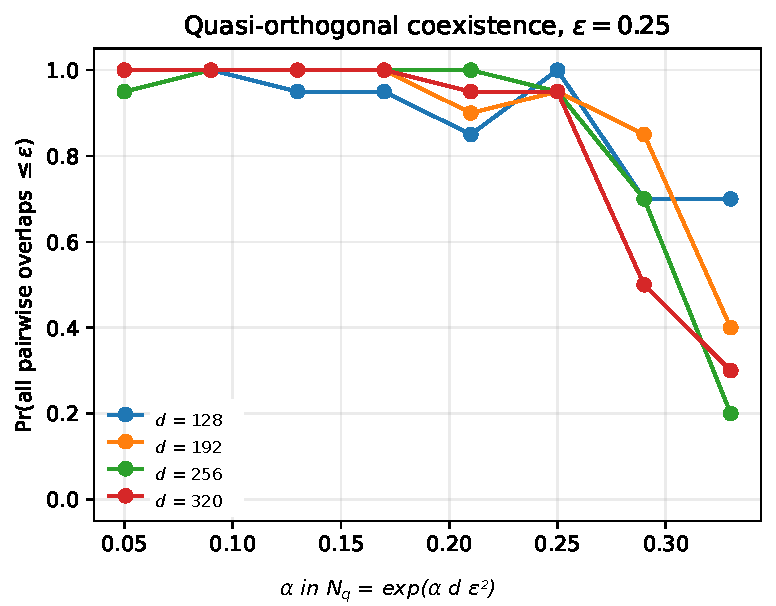
\includegraphics[width=0.48\textwidth]{2026-llm-quasi_orthogonal_coexistence.pdf}
\hfill
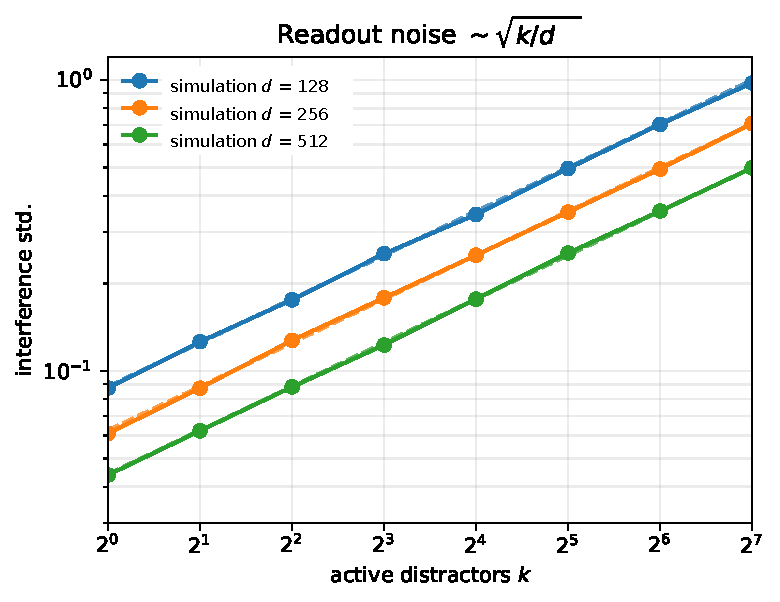
\includegraphics[width=0.48\textwidth]{2026-llm-readout_interference.pdf}
\caption{%
Synthetic geometry checks for the capacity/accessibility distinction.
Left: random unit directions in dimension $\deff$ are sampled with
$N=\exp(\alpha\,\deff\,\varepsilon^{2})$ and tested for
$\varepsilon$-quasi-orthogonality. For sufficiently small $\alpha$,
large families coexist with high probability, illustrating the
exponential packing side of Eq.~\eqref{eq:dual}. Right: for a fixed
target direction, $k$ random distractor directions are simultaneously
active with random signs. The standard deviation of the readout
interference follows the predicted scale
$\sint\sim\sqrt{k/\deff}$, illustrating the accessibility side of
Eq.~\eqref{eq:dual}. Both panels use random isotropic vectors and should
be read as a geometric null model rather than as measurements on a
trained language model.
}
\label{fig:toy-scalings}
\end{figure*}

This also clarifies the relation to compressed sensing. Stable recovery
of a $k$-sparse vector in an $N$-dimensional feature dictionary from
$m$ measurements typically requires
$m\gtrsim Ck\log(N/k)$ under suitable incoherence or restricted-isometry
assumptions~\cite{donoho2006compressed,candes2006robust,foucart2013mathematical}. In an idealized
isotropic residual stream, one may identify $m$ with $\deff$; in trained
models the effective representation dimension and effective readout
dimension may differ. The compressed-sensing analogy is therefore
diagnostic, not literal.

% ======================================================================
\section{Hinge vectors and sense subspaces}
\label{sec:hinge}
% ======================================================================

The previous section established an architecture-independent capacity
constraint. We now ask a more speculative question: how might a trained
model organize readout within that constraint? The hinge-and-frame
formalism is one possible answer. It is not implied by concentration
geometry, and it is separately falsifiable.

\subsection{The hinge hypothesis}
\label{sec:hingeform}

For a token $t$, let $v(t)\in\R^d$ be a candidate unit vector, called
a \emph{hinge}. Empirically this could be the static input embedding,
a mean contextual embedding, or a learned token-specific probe
direction. The hypothesis is not that every vector decomposition is
meaningful. Any state can be decomposed parallel and perpendicular to
any direction. The claim is stronger: for some tokens, a
token-associated direction is privileged relative to matched controls.

In the simplest case, given a context $C$, the hinge is the shared
first vector of a sense frame,
%
\begin{equation}
\label{eq:hinge-first}
e_1^C=v(t).
\end{equation}
%
The carrier for sense information is then the orthogonal complement
$v(t)^\perp$. A context selects a low-dimensional sense subspace
%
\begin{equation}
\label{eq:sense-subspace}
S^C=\spanop\{e_2^C,\dots,e_{q_C+1}^C\}
\subset v(t)^\perp ,
\end{equation}
%
with $q_C\ll\deff$ in the intended regime. For example,
$v(\text{bank})$ might be shared by finance, river, and aircraft-tilt
sense subspaces.

More generally, however, two contextual frames need not be interlinked
by only one shared atom. They may share a nontrivial link subspace
%
\begin{equation}
\label{eq:multi-hinge}
H_t=\spanop\{v_1(t),\dots,v_r(t)\},
\qquad r\ge 1 ,
\end{equation}
%
so that several token-associated directions are common to more than
one contextual frame. The single-hinge model corresponds to $r=1$.
For $r>1$, the sense carrier is $H_t^\perp$, and a contextual sense
subspace has the form
%
\begin{equation}
\label{eq:multi-sense-subspace}
S^C\subset H_t^\perp .
\end{equation}
%
This possibility is the semantic analogue of interlinked quantum
contexts sharing more than one common observable. In quantum logic,
such multiply interlinked contexts occur already in finite-dimensional
Hilbert-space configurations; for instance, two four-dimensional
contexts may be interconnected by two common link observables
\cite{svozil:040102}.

The low-rank assumption is empirical. A word sense is not a single
direction: it may involve topic, syntax, selectional preferences, and
world knowledge. But it should not need the full residual stream
either. The hinge hypothesis predicts that dominant within-sense
variation is low-dimensional after projection to the hinge-perpendicular
carrier, or more generally to the complement of the shared link
subspace. This prediction is compatible with existing evidence that
contextualized embeddings can separate word senses, but it is stronger:
it asks whether such separation is privileged relative to a
token-associated hinge or link subspace~\cite{wiedemann2019does,scarlini2020ares}.

\subsection{Gated-subspace readout}
\label{sec:gated}

Let $h(x)\in\R^d$ be the contextual state for input context $x$.
Relative to the hinge,
%
\begin{align}
\label{eq:hinge-decomp}
h(x)&=\hpar(x)v(t)+\hperp(x),
\\
\hpar(x)&=v(t)\T h(x),  \nonumber
\\
\hperp(x)&\in v(t)^\perp .  \nonumber
\end{align}
%
The scalar $\hpar$ measures engagement with the token-associated
direction. The perpendicular component $\hperp$ carries the
sense-disambiguating information. For a multi-link subspace $H_t$, the
same construction is obtained by replacing the scalar projection onto
$v(t)$ with the orthogonal projection onto $H_t$, and by taking the
carrier to be $H_t^\perp$.

Readout inside $S^C$ requires conditioning. Pairwise small overlaps are
not enough. Let
%
\begin{equation}
F_S^C=[\,e_2^C\ \cdots\ e_{q_C+1}^C\,],
\qquad
G_S^C=(F_S^C)\T F_S^C .
\end{equation}
%
We call the sense frame $\rho$-stable if
%
\begin{equation}
\label{eq:rho-stable}
\opnorm{G_S^C-I}\le \rho<1 .
\end{equation}
%
Then the dual frame
%
\begin{equation}
\label{eq:dual-frame}
\widetilde F_S^C=F_S^C(G_S^C)^{-1}
\end{equation}
%
is well-defined and satisfies
$\opnorm{\widetilde F_S^C}\le(1-\rho)^{-1/2}$. Near-degenerate frames
amplify readout noise; the model requires $\rho$ comfortably below one.

The dual-frame coefficients are
%
\begin{equation}
\label{eq:alpha}
\alpha^C(x)=\bigl(\widetilde F_S^C\bigr)\T\hperp(x)
\in\R^{q_C}.
\end{equation}
%
A simple sense score is
%
\begin{equation}
\label{eq:sense-score}
s_C(x)=g(\hpar(x))\,r_C(\hperp(x)),
\end{equation}
%
where $g\ge0$ is an engagement gate and $r_C\ge0$ measures how well
$\hperp(x)$ fits the sense subspace. One may take
$r_C=\norm{\alpha^C(x)}^2$, a squared overlap with a distinguished
direction in $S^C$, or a learned positive quadratic form. The selected
sense frame is
%
\begin{equation}
\label{eq:selected-frame}
C^*(x)=\argmax_C s_C(x).
\end{equation}
%
The precise gate is not essential. The empirical content is the
separation: the parallel coordinate gates token engagement; the
perpendicular carrier contains sense information.

The hinge matters because different candidate hinges induce different
carriers. Likewise, different candidate link subspaces induce different
orthogonal carriers. If no token-associated hinge or link subspace
exposes sense structure better than matched random or
frequency-controlled directions, the hinge hypothesis fails.

Figure~\ref{fig:hinge} illustrates the minimal single-link case for the
polysemous token ``bank.'' The shared vector
$\bm v(\text{bank})$ is the candidate hinge. The vectors
$\bm w^{\mathcal C_{\rm fin}}$,
$\bm w^{\mathcal C_{\rm riv}}$, and
$\bm w^{\mathcal C_{\rm tilt}}$ denote representative directions inside
the corresponding sense subspaces
$S^{\mathcal C_{\rm fin}}$,
$S^{\mathcal C_{\rm riv}}$, and
$S^{\mathcal C_{\rm tilt}}$. They are not meant to exhaust those
subspaces; they merely mark one salient direction in each contextual
frame.

\begin{figure}[t]
\centering
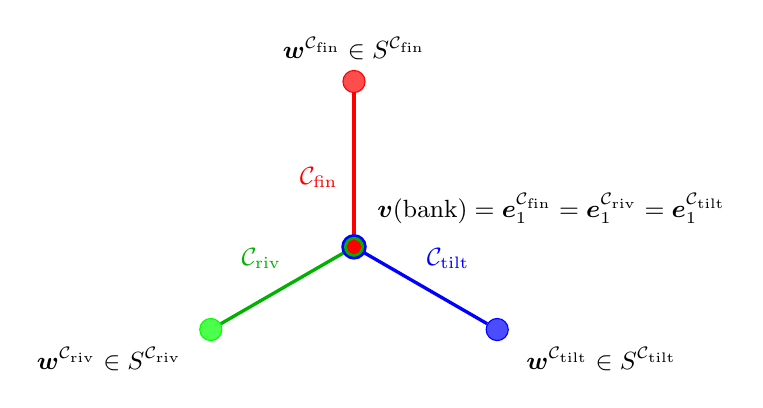
\begin{tikzpicture}[scale=0.5,
    outer/.style={circle, draw, minimum size=8pt,
                  inner sep=0pt, font=\footnotesize},
    lab/.style={font=\small}]
% central shared vector
\coordinate (c) at (0,0);

\node[lab, above right=7pt] at (c)
{$\bm{v}(\text{bank})
=\bm{e}_1^{\mathcal{C}_{\rm fin}}
=\bm{e}_1^{\mathcal{C}_{\rm riv}}
=\bm{e}_1^{\mathcal{C}_{\rm tilt}}$};

% outer distinguishing vectors
\node[outer, red, fill=red!70,
      label={[lab]above:
      $\bm{w}^{\mathcal{C}_{\rm fin}}
      \in S^{\mathcal{C}_{\rm fin}}$}]
      (fin) at (90:4.2cm) {};

\node[outer, green, fill=green!70,
      label={[lab, xshift=-4pt]below left:
      $\bm{w}^{\mathcal{C}_{\rm riv}}
      \in S^{\mathcal{C}_{\rm riv}}$}]
      (riv) at (210:4.2cm) {};

\node[outer, blue, fill=blue!70,
      label={[lab, xshift=4pt]below right:
      $\bm{w}^{\mathcal{C}_{\rm tilt}}
      \in S^{\mathcal{C}_{\rm tilt}}$}]
      (tilt) at (330:4.2cm) {};

% edges labelled by contextual frames
\draw[very thick, red] (c) --
      node[lab, left=2pt, pos=0.45]
      {$\mathcal{C}_{\rm fin}$} (fin);

\draw[very thick, green!70!black] (c) --
      node[lab, above left=1pt, pos=0.45]
      {$\mathcal{C}_{\rm riv}$} (riv);

\draw[very thick, blue] (c) --
      node[lab, above right=1pt, pos=0.45]
      {$\mathcal{C}_{\rm tilt}$} (tilt);

% central concentric disks
\filldraw[blue, very thick] (c) circle (8pt);
\filldraw[green!70!black, very thick] (c) circle (6pt);
\filldraw[red, very thick] (c) circle (4pt);
\end{tikzpicture}
\caption{%
Schematic of hinge-anchored frame sharing in the simplest
single-link case. A candidate hinge vector associated with the token
``bank'' is shared by several possible sense frames. The colored outer
nodes represent exemplary directions
$\bm w^{\mathcal C_{\rm fin}}$,
$\bm w^{\mathcal C_{\rm riv}}$, and
$\bm w^{\mathcal C_{\rm tilt}}$ inside the corresponding sense
subspaces, not the entire subspaces themselves. The formal model treats
sense content as lying in low-dimensional subspaces of the
hinge-perpendicular carrier $\bm v(\text{bank})^\perp$. More generally,
two contextual frames may share several link directions, in which case
the relevant carrier is the orthogonal complement of the shared link
subspace rather than of a single hinge vector.
}
\label{fig:hinge}
\end{figure}

\subsection{Packing sense subspaces around one hinge}
\label{sec:grassmann}

The vector packing bound extends to low-dimensional subspaces. Fix a
unit vector $v_0\in\Sph{d-1}$ and let $m=d-1$. For $1\le q\ll m$ and
any fixed threshold $\mu>2\sqrt{q/m}$, there exist
$q$-dimensional subspaces
$S_1,\dots,S_M\subset v_0^\perp$ such that
%
\begin{equation}
\label{eq:grassmann-coherence}
\opnorm{U_a\T U_b}\le \mu,\qquad a\neq b,
\end{equation}
%
where $U_a,U_b\in\R^{m\times q}$ are orthonormal basis matrices, and
%
\begin{equation}
\label{eq:grassmann-count}
M\ge \exp(c_{\mu,q}m)
\end{equation}
%
for some positive $c_{\mu,q}$.

This is a standard Grassmannian packing consequence of concentration
on Stiefel and Grassmann manifolds~\cite{szarek1982nets,conway1996packings}. For
two independent Haar-random $q$-planes, the singular values of
$U\T V$ are the cosines of their principal angles. In the regime
$q\ll m$, the largest principal correlation is of order
$\sqrt{q/m}$~\cite{chikuse2003statistics,absil2006condition,edelman1998random}. A union bound
over sampled subspaces then gives an exponential packing.

For trained representations this statement must be read inside an
approximately isotropic effective carrier of dimension
$\meff=\deff-1$, not necessarily inside the raw ambient space. More
generally, if the shared link subspace has dimension $r$, the relevant
carrier dimension is $\meff=\deff-r$. Without such an effective
carrier, the Haar-random subspace model is not a good description of
activation geometry.

\subsection{Relation to dynamic contextual embeddings}
\label{sec:dynamic}

Transformers already handle polysemy dynamically. The state
$h_\ell(t\mid x)$ of token $t$ at layer $\ell$ depends on context $x$.
The hinge formalism is not an alternative architecture; it is a
possible decomposition of such trajectories.

Given a candidate hinge $h_t$, write
%
\begin{align}
\label{eq:layer-decomp}
h_\ell(t\mid x)
&=
a_\ell(t,x)h_t+z_\ell(t,x),
\\
a_\ell(t,x)&=h_t\T h_\ell(t\mid x),\nonumber
\\
z_\ell(t,x)&\in h_t^\perp .\nonumber
\end{align}
%
The decomposition is trivial; the hypothesis is not. Hinge anchoring
predicts that $a_\ell$ tracks token engagement or salience, while
$z_\ell$ carries most sense-disambiguating information. Sense labels
should become more separable in $h_t^\perp$ than in the orthogonal
complements of matched control directions. For each sense $s$, the
vectors $z_\ell(t,x)$ should also concentrate near a low-dimensional
subspace $S_s\subset h_t^\perp$. In the multi-link variant, $h_t^\perp$
is replaced by the orthogonal complement of the candidate link subspace
$H_t$.

Thus the critical question is not whether contextual embeddings move;
they do. The question is whether their movement has a privileged
hinge-perpendicular, or more generally link-complement, organization.

\begin{table*}[ht]
\caption{Dynamic contextual embeddings versus the hinge-decomposition
hypothesis.}
\label{tab:two-views}
\centering
\begin{minipage}{0.68\textwidth}
\begin{ruledtabular}
\begin{tabular}{@{}ll@{}}
Dynamic description & Hinge-decomposition hypothesis \\
\colrule
Token state changes by context and layer & State decomposes relative to a hinge \\
Layer activation carries context & Hinge-perpendicular part carries sense \\
Polysemy by vector deformation & Polysemy by gated subspace readout \\
Resource is depth and width & Resource is quasi-dimensionality \\
Limit is activation bottleneck & Limit is interference/accessibility \\
\end{tabular}
\end{ruledtabular}
\end{minipage}
\end{table*}

% ======================================================================
\section{Attention and latent frame selection}
\label{sec:attention}
% ======================================================================

A standard attention head computes
%
\begin{equation}
\label{eq:attention}
h'=\sum_j\alpha_j\nu_j,
\qquad
\alpha_j=
\frac{\exp(q\T k_j/\sqrt d)}
{\sum_{j'}\exp(q\T k_{j'}/\sqrt d)} .
\end{equation}
%
Keys and values are produced by different learned maps, so values are
not generally dual-frame coefficients for keys. Attention is therefore
not literal dual-frame reconstruction.

The useful analogy is softer. Attention routes information: it
amplifies some contextual directions and suppresses others. In the
hinge language, this resembles subspace or frame selection. A literal
dual-frame interpretation would require additional constraints, such
as approximately Parseval keys and values implementing the corresponding
dual reconstruction. We do not assume this.

A compact latent-variable version is
%
\begin{equation}
\label{eq:latent}
p(t\mid x)=\sum_C p(t\mid x,C)\,p(C\mid x),
\end{equation}
%
where $C$ indexes candidate contextual frames. One may model
%
\begin{equation}
\label{eq:frame-temp}
p(C\mid x)=
\frac{\exp(s_C(x)/T)}
{\sum_{C'}\exp(s_{C'}(x)/T)} ,
\end{equation}
%
with $s_C$ the gated score of Eq.~\eqref{eq:sense-score}. This is not
a claim about the literal implementation of decoding in current LLMs:
standard temperature acts on token logits, not on explicit latent
frames. The point is only that ambiguity can be represented as a
distribution over possible readout frames rather than as a single fixed
interpretation.

% ======================================================================
\section{Discussion}
\label{sec:discussion}
% ======================================================================

The main proposal is the capacity/accessibility distinction. The hinge
formalism is a possible organization within that constraint, not a
consequence of it.

\subsection{Relation to superposition and sparse autoencoders}
\label{sec:superposition}

The superposition hypothesis holds that neural networks represent more
features than they have neurons by packing features into nearly
orthogonal directions~\cite{elhage2022superposition,bricken2023monosemanticity}. The concentration
estimate~\eqref{eq:overlap} gives the kinetic side of that picture:
many directions can coexist. Equation~\eqref{eq:sint} gives the
epistemic side: many jointly active features create interference of
scale $\sqrt{k/\deff}$. Sparsity is therefore not an implementation
detail; it is necessary for readout.

Sparse autoencoders (SAEs) give a concrete empirical interface. They
approximate layer activations as sparse expansions over learned decoder
directions, making the $w_i$ of Eq.~\eqref{eq:hidden} measurable
objects rather than hypothetical features. Recent work has scaled SAEs,
studied SAE feature geometry, and automated interpretation of large
numbers of latents~\cite{gao2025scaling,li2025geometry,paulo2025automatically,shu2025survey}. In the
present framework, SAE decoder directions can test the
capacity/accessibility prediction, while sense-conditioned SAE
activation clusters can test the stronger hinge hypothesis.

\subsection{A coactivation-weighted capacity limit}
\label{sec:capacity-limit}

The active-set size $k$ is a crude summary. A more refined description
uses the coactivation graph
%
\begin{equation}
\label{eq:coactivation}
C_{ij}=\Prob(i,j\text{ active}).
\end{equation}
%
If active amplitudes have, conditional on coactivation, zero mean and
pairwise uncorrelated signs, then cross terms cancel in expectation and
feature $j$ contributes to the readout variance of feature $i$ in
proportion to
$\E[x_j^2\mid i,j\text{ active}](w_i\T w_j)^2$. Absorbing amplitude
variance and feature importance into coefficients $a_i,a_j$ gives
%
\begin{equation}
\label{eq:int-energy}
\Eint=
\sum_{i\neq j}
C_{ij}a_i a_j (w_i\T w_j)^2 .
\end{equation}
%
Frequently coactive features are therefore pressured toward
orthogonality. Rarely coactive or mutually exclusive features are much
less constrained and may share directions or even become approximately
antipodal if nonlinear readout makes this useful. The relevant object
is not just the number of features, but the weighted coactivation graph.

\subsection{Limitations}
\label{sec:limitations}

The framework can fail in several ways.

First, anisotropy may make $\deff$ much smaller than $d$.
Contextual embeddings are known to be anisotropic, and intrinsic
dimension can vary strongly by layer and training regime
\cite{ethayarajh2019,gao2019representation,mu2018allbutthetop,razzhigaev2024shape}. Whitening and
related postprocessing can partially restore isotropic geometry
\cite{gao2019representation,mu2018allbutthetop,su2021whitening}. At the same time, anisotropy should not
be treated as an automatic or universal property of all Transformer
representations~\cite{machina2024anisotropy}. The bounds should always
be read in terms of the effective dimension actually achieved.

Second, the hinge readout needs well-conditioned sense frames. If
$\rho$ in Eq.~\eqref{eq:rho-stable} is close to one, the dual-frame
readout amplifies noise.

Third, the hinge pattern may simply be descriptively wrong. Trained
models may represent polysemy without any preferred token-associated
direction or link subspace. In that case the capacity/accessibility
account may still hold, but the hinge hypothesis fails.

Fourth, the law $\sint\sim\sqrt{k/\deff}$ assumes random-like
incoherent directions and weakly correlated signs or amplitudes.
Learned networks may improve on this by orthogonalizing frequently
coactive features, or worsen it through anisotropy and correlated
errors. The law is a scaling principle, not a universal equality.

Finally, the hinge formalism has modeling choices: the hinge or link
subspace, the gate, the selector, and the sense-subspace dimension.
These choices must be fixed or controlled empirically. Otherwise the
framework risks describing whatever geometry is found after the fact.

\subsection{Empirical predictions}
\label{sec:predictions}

The key empirical task is to separate the general capacity claim from
the stronger hinge claim.

{Claim A: hinge anchoring.}
For a polysemous token $t$, there exists a privileged token-associated
direction $h_t$, or more generally a privileged token-associated link
subspace $H_t$, such that sense-relevant variation is better exposed in
the corresponding orthogonal carrier than in the orthogonal complements
of matched control directions or subspaces.

{Claim B: low-dimensional sense frames.}
Within $h_t^\perp$, or more generally within $H_t^\perp$,
sense-conditioned states concentrate near low-dimensional subspaces
with small cross-sense coherence.

These claims can fail independently. Claim A can hold while sense
information remains high-dimensional. Claim B can hold relative to some
non-token-associated direction or subspace, in which case hinge
anchoring fails.

The following tests separate the possibilities.

\begin{enumerate}
\item \emph{Hinge-anchoring test.}
For a polysemous token, choose candidate hinges such as the static input
embedding, mean contextual embedding, or a learned token-specific
direction. Decompose layer states as in Eq.~\eqref{eq:layer-decomp}.
Sense labels should be better separated in $h_t^\perp$ than in
orthogonal complements of random, frequency-matched, or layer-matched
control directions. The statistic may be classification accuracy or
mutual information with sense labels, assessed by permutation over
sense labels and bootstrap over token instances. The same test can be
run for candidate link subspaces $H_t$ by replacing $h_t^\perp$ with
$H_t^\perp$.

\item \emph{Operational subspace test.}
For each sense $s$, collect projected states
$z_\ell(t,x)\in h_t^\perp$ and estimate a low-rank subspace by PCA or
probabilistic factor analysis. With $U_s$ the first $q$ principal
directions, measure cross-sense coherence
$\opnorm{U_s\T U_{s'}}$. True sense labels should yield lower
cross-sense coherence than shuffled labels and stronger separation than
control hinges. In the multi-link variant, the same procedure is
performed after projection to $H_t^\perp$.

\item \emph{Gated-readout test.}
Linear probes trained on $z_\ell(t,x)$ should perform comparably to
probes trained on the full state $h_\ell(t\mid x)$, while probes
restricted to the parallel component $a_\ell(t,x)h_t$ should perform
near chance on sense classification.

\item \emph{Overlap-distribution test.}
If a representation exploits quasi-dimensionality, pairwise inner
products among token embeddings or SAE feature directions should
concentrate near zero with variance $\sim1/\deff$. Deviations quantify
anisotropy and effective dimension loss.

\item \emph{Synthetic concurrency degradation.}
At a fixed layer, inject controlled superpositions
%
\begin{equation}
h_k=h_0+\lambda\sum_{j=1}^k x_j w_j,
\end{equation}
%
using directions $w_j$ obtained independently, for example from SAE
decoder directions or frozen linear probes. As $k$ increases, readout
should degrade smoothly on the scale $\sqrt{k/\deff}$ for random-like
directions, with weaker degradation for feature sets that training has
orthogonalized.

\item \emph{Coactivation-dependent geometry.}
Frequently coactive features should show reduced mutual coherence
relative to rarely coactive features. This tests the broader
capacity/accessibility framework through Eq.~\eqref{eq:int-energy},
independently of the hinge hypothesis.
\end{enumerate}

\subsection{Scope of the quantum analogy}
\label{sec:quantum}

The analogy to quantum contextuality is structural and limited. Both
settings involve vectors whose operational role depends on a frame.
But quantum contextuality has the force of no-go theorems such as
Kochen--Specker~\cite{specker-60,kochen1}; no analogous theorem is
claimed here for semantic embeddings. The borrowed idea is only the
shared-vector frame structure: one or more vectors may participate in
several possible frames, and readout depends on which frame is selected.

The qualifier ``one or more'' is important. In Hilbert-space quantum
logic, different contexts can be interlinked by a single common
observable, as in the familiar tripod-like case, but also by several
common observables. A four-dimensional example consists of two contexts
interconnected by two link observables~\cite{svozil:040102}.
The semantic analogue is that a token need not possess only a single
hinge direction. A family of related senses may share a
higher-dimensional link subspace $H_t$, with sense-specific information
carried in subspaces of $H_t^\perp$. Thus the single-hinge picture
should be read as the minimal case, not as a structural necessity.

% ======================================================================
\section{Conclusion}
\label{sec:conclusion}
% ======================================================================

High-dimensional representations can host many semantic possibilities,
but finite readout limits how many can be made simultaneously
accessible. The main quantitative content is the same pair of scalings
introduced in Eqs.~\eqref{eq:intro-capacity} and~\eqref{eq:intro-readout}:
%
\begin{equation}
\label{eq:summary}
N\lesssim\exp(c\,\deff\,\varepsilon^{2}),
\qquad
\sint\sim\sqrt{k/\deff}.
\end{equation}
%
The first expression is a coexistence bound; the second is a readout
noise scale. They are not the same kind of theorem, but together they
describe the difference between semantic capacity and semantic
accessibility.

Within this framework we proposed the hinge-and-frame hypothesis: some
polysemous tokens may be organized around stable token-associated
directions, or more generally around token-associated link subspaces,
with sense information encoded in low-dimensional subspaces of the
orthogonal carrier. This hypothesis is not forced by geometry. Its
critical test is whether token-associated hinges or link subspaces
expose sense structure better than matched controls. A negative result
would falsify hinge anchoring while leaving the broader superposition
and interference picture intact.

\begin{acknowledgments}
This work was supported in part by the Austrian Science Fund (FWF)
Grant DOI: 10.55776/PIN5424624. Portions of the manuscript were drafted
with assistance from large language models; all ideas, arguments, and
final formulations are the author's responsibility.
\end{acknowledgments}

\bibliography{svozil}

\end{document}
